\section{Counting lattice diameter lines}\label{sec:QP}

Ehrhart theory studies the number of lattice points in dilations of a given lattice (or rational) polytope. A fundamental result by Ehrhart states that this counting function agrees with a polynomial function for lattice polytopes, and a quasi-polynomial function for rational polytopes. For details, see \cite{beckrobins}. In this section we show that for lattice polygons $P$ the counting function $\LD_P(k)$, which counts the number of lattice diameter lines (or segments) in the dilate $kP$, agrees with a quasi-polynomial function.

\begin{example}\label{ex:qp}
    Let $P= \conv(\{(0,0), (1,3), (5,1), (6,4)\})$. In \Cref{fig:dilations} we depict the segments $L \cap P$ for lattice diameter lines $L$ of $kP$ for $k=1, \ldots, 6$.
    
    %\input{Figures/2.30_dilations.tex}
\begin{figure}[ht!]
    \centering
    %\includegraphics[width=\linewidth]{Figures/2.30_dilations.png}
    \tikzset{every picture/.style={line width=0.75pt}} % ancho por defecto

\begin{tikzpicture}[x=0.75pt,y=0.75pt,yscale=-.3,xscale=.3]


% ---------- Estilos ----------
\tikzset{
  graydot/.style={circle, draw=lightgray, fill=lightgray, minimum width=1pt, inner sep=0pt},
  sone/.style={circle, draw={rgb,255:red,245;lightgreen,166;blue,35}, fill={rgb,255:red,245;lightgreen,166;blue,35}, minimum width=1pt, inner sep=0pt}, % naranja (S1)
  stwo/.style={circle, draw={rgb,255:red,144;lightgreen,19;blue,254},  fill={rgb,255:red,144;lightgreen,19;blue,254},  minimum width=1pt, inner sep=0pt}  % morado (S2)
}



% ==================================================
% MALLA 1 (izquierda)
% ==================================================
\pgfmathsetmacro{\XL}{460}
\pgfmathsetmacro{\YL}{180}
\foreach \i in {0,...,6}{
  \foreach \j in {0,...,4}{
    \node[graydot] at ({\XL + 20*\i},{\YL + 20*\j}) {};
  }
}
% Quadrilateros
\foreach \j in {0}{
  \pgfmathsetmacro{\XL}{460+\j*20}
  \pgfmathsetmacro{\YL}{180-\j*60}
  \foreach \i in {0}{
    \draw [color=black, draw opacity=1]
  (\XL+\i*100,\YL+80-\i*20)  -- (\XL+100+\i*100,\YL+60-\i*20) -- (\XL+120+\i*100,\YL-\i*20) --(\XL+20+\i*100,\YL+20-\i*20) -- cycle;
  }
}

% Dibujar líneas naranjas paralelas
\draw[color=orange, line width=.8pt, draw opacity=1] (478, 200) -- (576, 200);
\draw[color=orange, line width=.8pt, draw opacity=1] (471, 220) -- (569, 220);
\draw[color=orange, line width=.8pt, draw opacity=1] (464, 240) -- (562, 240);

  

% ==================================================
% MALLA 2 (medio)  ---- puntos grises con bucle
% ==================================================
\pgfmathsetmacro{\XL}{1020}
\pgfmathsetmacro{\YL}{140}
\foreach \i in {0,...,12}{
  \foreach \j in {0,...,8}{
    \node[graydot] at ({\XL + 20*\i},{\YL + 20*\j}) {};
  }
}

% Quadrilateros
\foreach \j in {0,1}{
  \pgfmathsetmacro{\XL}{1020+\j*20}
  \pgfmathsetmacro{\YL}{220-\j*60}
  \foreach \i in {0,1}{
    \draw [color=black, draw opacity=1]
  (\XL+\i*100,\YL+80-\i*20)  -- (\XL+100+\i*100,\YL+60-\i*20) -- (\XL+120+\i*100,\YL-\i*20) --(\XL+20+\i*100,\YL+20-\i*20) -- cycle;
  }
}

% Dibujar líneas moradas paralelas
\draw[color=darklav, line width=.8pt, draw opacity=1] (1056, 180) -- (1247.61, 180);
\draw[color=darklav, line width=.8pt, draw opacity=1] (1051, 200) -- (1242.61, 200);
\draw[color=darklav, line width=.8pt, draw opacity=1] (1037, 240) -- (1229.61, 240);
\draw[color=darklav, line width=.8pt, draw opacity=1] (1030, 260) -- (1222.61, 260);

% ==================================================
% MALLA 3 (derecha)  ---- puntos grises con bucle
% ==================================================
\pgfmathsetmacro{\Xo}{1680}
\pgfmathsetmacro{\Yo}{110}
\foreach \i in {0,...,18}{
  \foreach \j in {0,...,12}{
    \node[graydot] at ({\Xo + 20*\i},{\Yo + 20*\j}) {};
  }
}

% Quadrilateros
\foreach \j in {0,1,2}{
  \pgfmathsetmacro{\XL}{1680+\j*20}
  \pgfmathsetmacro{\YL}{270-\j*60}
  \foreach \i in {0,1,2}{
    \draw [color=black, draw opacity=1]
  (\XL+\i*100,\YL+80-\i*20)  -- (\XL+100+\i*100,\YL+60-\i*20) -- (\XL+120+\i*100,\YL-\i*20) --(\XL+20+\i*100,\YL+20-\i*20) -- cycle;
  }
}

\draw[color=lightgreen, line width=.8pt, draw opacity=1] (1740, 170) -- (2020, 170);
\draw[color=lightgreen, line width=.8pt, draw opacity=1] (1720, 230) -- (2000, 230);
\draw[color=lightgreen, line width=.8pt, draw opacity=1] (1700, 290) -- (1980, 290);


% ==================================================
% MALLA 4 (izquierda) ---- puntos grises con bucle
% ==================================================
\pgfmathsetmacro{\XL}{290}
\pgfmathsetmacro{\YL}{600}
\foreach \i in {0,...,24}{
  \foreach \j in {0,...,16}{
    \node[graydot] at ({\XL + 20*\i},{\YL + 20*\j}) {};
  }
}

% Quadrilateros
\foreach \j in {0,...,3}{
  \pgfmathsetmacro{\XL}{290+\j*20}
  \pgfmathsetmacro{\YL}{840-\j*60}
  \foreach \i in {0,...,3}{
    \draw [color=black, draw opacity=1]
  (\XL+\i*100,\YL+80-\i*20)  -- (\XL+100+\i*100,\YL+60-\i*20) -- (\XL+120+\i*100,\YL-\i*20) --(\XL+20+\i*100,\YL+20-\i*20) -- cycle;
  }
}

% Dibujar líneas naranjas paralelas
\draw[color=orange, line width=.8pt, draw opacity=1] (371, 680) -- (745.61, 680);
\draw[color=orange, line width=.8pt, draw opacity=1] (364, 700) -- (738.61, 700);
\draw[color=orange, line width=.8pt, draw opacity=1] (357, 720) -- (731.61, 720);
\draw[color=orange, line width=.8pt, draw opacity=1] (350, 740) -- (724.61, 740);
\draw[color=orange, line width=.8pt, draw opacity=1] (343, 760) -- (717.61, 760);
\draw[color=orange, line width=.8pt, draw opacity=1] (336, 780) -- (710.61, 780);
\draw[color=orange, line width=.8pt, draw opacity=1] (329, 800) -- (703.61, 800);
\draw[color=orange, line width=.8pt, draw opacity=1] (322, 820) -- (696.61, 820);
\draw[color=orange, line width=.8pt, draw opacity=1] (315, 840) -- (689.61, 840);


% ==================================================
% MALLA 5 (medio)  ---- puntos grises con bucle
% ==================================================
\pgfmathsetmacro{\Xo}{850}
    \pgfmathsetmacro{\Yo}{560}
\foreach \i in {0,...,30}{
  \foreach \j in {0,...,20}{
    \node[graydot] at ({\Xo + 20*\i},{\Yo + 20*\j}) {};
  }
}


% Quadrilateros
\foreach \j in {0,...,4}{
  \pgfmathsetmacro{\XL}{850+\j*20}
  \pgfmathsetmacro{\YL}{880-\j*60}
  \foreach \i in {0,...,4}{
    \draw [color=black, draw opacity=1]
  (\XL+\i*100,\YL+80-\i*20)  -- (\XL+100+\i*100,\YL+60-\i*20) -- (\XL+120+\i*100,\YL-\i*20) --(\XL+20+\i*100,\YL+20-\i*20) -- cycle;
  }
}

% Dibujar líneas moradas paralelas
\draw[color=darklav, line width=.8pt, draw opacity=1] (948, 660) -- (1417.61, 660);
\draw[color=darklav, line width=.8pt, draw opacity=1] (943, 680) -- (1412.61, 680);
\draw[color=darklav, line width=.8pt, draw opacity=1] (929, 720) -- (1399.61, 720);
\draw[color=darklav, line width=.8pt, draw opacity=1] (922, 740) -- (1392.61, 740);
\draw[color=darklav, line width=.8pt, draw opacity=1] (908, 780) -- (1378.61, 780);
\draw[color=darklav, line width=.8pt, draw opacity=1] (901, 800) -- (1371.61, 800);
\draw[color=darklav, line width=.8pt, draw opacity=1] (888, 840) -- (1357.61, 840);
\draw[color=darklav, line width=.8pt, draw opacity=1] (883, 860) -- (1353.61, 860);


% ==================================================
% MALLA 6 (derecha)  ---- puntos grises con bucle
% ==================================================
\pgfmathsetmacro{\Xo}{1540}
\pgfmathsetmacro{\Yo}{520}
\foreach \i in {0,...,36}{
  \foreach \j in {0,...,24}{
    \node[graydot] at ({\Xo + 20*\i},{\Yo + 20*\j}) {};
  }
}

% Quadrilateros
\foreach \j in {0,...,5}{
  \pgfmathsetmacro{\XL}{1540+\j*20}
  \pgfmathsetmacro{\YL}{920-\j*60}
  \foreach \i in {0,...,5}{
    \draw [color=black, draw opacity=1]
  (\XL+\i*100,\YL+80-\i*20)  -- (\XL+100+\i*100,\YL+60-\i*20) -- (\XL+120+\i*100,\YL-\i*20) --(\XL+20+\i*100,\YL+20-\i*20) -- cycle;
  }
}

% Dibujar líneas moradas paralelas

\draw[color=lightgreen, line width=.8pt, draw opacity=1] (1662, 640) -- (2224, 640);
\draw[color=lightgreen, line width=.8pt, draw opacity=1] (1642, 700) -- (2204, 700);
\draw[color=lightgreen, line width=.8pt, draw opacity=1] (1622, 760) -- (2184, 760);
\draw[color=lightgreen, line width=.8pt, draw opacity=1] (1600, 820) -- (2164, 820);
\draw[color=lightgreen, line width=.8pt, draw opacity=1] (1582, 880) -- (2144, 880);








% Text Node
\draw (490,300) node [anchor=north west][inner sep=0.75pt]    {$P$};
% Text Node
\draw (1120,335) node [anchor=north west][inner sep=0.75pt]    {$2P$};
% Text Node
\draw (1840,385) node [anchor=north west][inner sep=0.75pt]    {$3P$};
% Text Node
\draw (480,960) node [anchor=north west][inner sep=0.75pt]    {$4P$};
% Text Node
\draw (1120,1010) node [anchor=north west][inner sep=0.75pt]    {$5P$};
% Text Node
\draw (1840,1050) node [anchor=north west][inner sep=0.75pt]    {$6P$};



\end{tikzpicture}

    \caption{The pattern of lattice diameter lines repeats periodically under dilation of $P$.}
    \label{fig:dilations}
\end{figure}

    Then for all $k \in \N$ we get\vspace{-1em}
    \begin{align*}
        \LD_P(k)=\begin{cases}
            2k+1 & \text{if } k \equiv 1 \pmod 3,\\
            \frac{4}{3} k + \frac{4}{3} & \text{if } k \equiv 2 \pmod 3,\\
            \frac{2}{3} k + 1 & \text{if } k \equiv 0 \pmod 3.
        \end{cases}
    \end{align*}
    Indeed, $\LD_P(1)=3,\ \LD_P(2)=4,\ \LD_P(3)=3,\ \LD_P(4)=9,\ \LD_P(5)=8$ and $\LD_P(6)=5$.
\end{example}

For a set $X \subseteq \R^d$ we write $kX:= \{k \bx \st \bx \in X\}$ for the dilated set by $k \in \N$. In particular, for a polytope $P$, any line intersecting $kP$ can be written as the dilated line $kL$ for a \mbox{line $L$ intersecting $P$.}

\begin{lemma}\label{lemma:same-dir}
    Let $P$ be a lattice polygon and let $k \in \N$. Then, a diameter direction of $kP$ is also a diameter direction of $P$.
\end{lemma}
\begin{proof}
    Let $\bu$ be a diameter direction of $kP$ and let $kL$ be a lattice diameter line with direction $\bu$ that passes through a vertex of $kP$. (That is, $L$ is a line that passes through the corresponding vertex of $P$). Let $L'$ be a lattice line that passes through a vertex of $P$. Then, $kL'$ also passes through a vertex of $kP$ and by \Cref{lem:nvol}
    \begin{align}\label{eq:diam-dir-stay}
        \lfloor \nvol(kL \cap kP) \rfloor +1 = |kL \cap kP \cap \Z^2|  \geq |kL' \cap kP \cap \Z^2| = \lfloor \nvol(kL' \cap kP) \rfloor +1.
    \end{align}
    The normalized volume is a homogeneous function in $k$, so \eqref{eq:diam-dir-stay} and \Cref{lem:nvol} yield
    %since $L,L'$ pass through vertices of $P$ we get
    \begin{align*}
        |L \cap P \cap \Z^2|  = \lfloor \nvol(L \cap P) \rfloor +1 \geq \lfloor \nvol(L' \cap P) \rfloor +1 =|L' \cap P \cap \Z^2|.
    \end{align*}
    Since for every diameter direction of $P$ there exists a lattice diameter line in that direction, that passes through a vertex, we proved that $L$ is a lattice diameter line of $P$. In particular, $\bu$ is a diameter direction of $P$.
\end{proof}

% The next lemma says that only some lattice diameter segments ``remain'' a lattice diameter segment under dilation of the polygon, precisely those for which $L \cap P$ has largest normalized length. \Cref{fig:nvol-dom} illustrates this phenomenon.
The following lemma shows that under dilation of the polygon only certain lattice diameter lines remain, specifically those for which $L \cap P$ has the largest normalized length. \Cref{fig:nvol-dom} illustrates this phenomenon.

%dilated polytope 3x where ldsegments disappear

\begin{figure}[ht!]
    \centering
    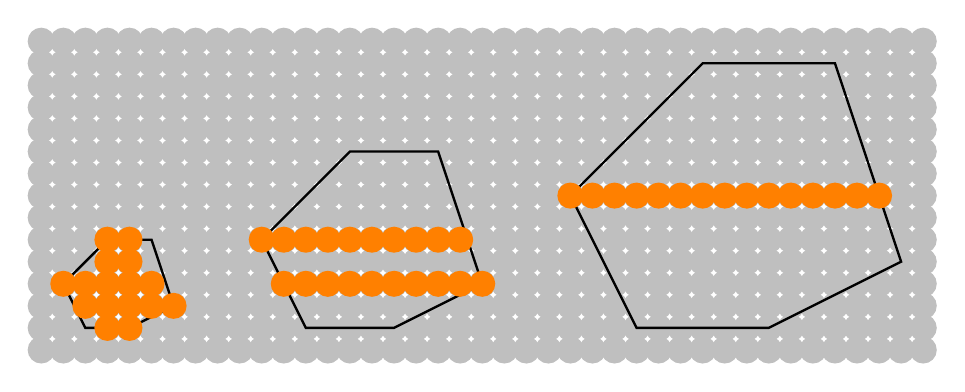
\begin{tikzpicture}[thin, scale=0.28]\vspace{0.5cm}
        \foreach \x in {-4,...,36} {
            \foreach \y in {-1,...,13} {
                \node at (\x,\y) [circle, draw=lightgray, fill= lightgray, minimum width=1.5pt] {};   
            }
        }
    
    %Outline of polytopes 1P, 2P, 3P
    \draw[line width=0.3mm, black] (-2,0) -- (-3,2) --(-1,4) --(1,4) -- (2,1)-- (0,0) -- cycle;
    \draw[line width=0.3mm, black](8,0) -- (6,4) -- (10,8) -- (14,8) -- (16,2) -- (12,0) -- cycle;
    \draw[line width=0.3mm, black] (23,0) -- (20,6) -- (26,12) -- (32,12) -- (35,3) -- (29,0) -- cycle;

    
    %Lattice Diameters in P
    %full segments L \cap P
    % \draw[line width=0.3mm, orange] (-3,2) -- (1.66,2);
    % \draw[line width=0.3mm, orange] (-2.5,1) -- (2,1);
    
    %ends at last lattice point
    \draw[line width=0.3mm, orange] (-3,2) -- (1,2);
    \draw[line width=0.3mm, orange] (-2,1) -- (2,1);
    
    %same for both
    \draw[line width=0.3mm, orange] (-1,0) -- (-1,4);
    \draw[line width=0.3mm, orange] (0,0) -- (0,4);

     \foreach \x in {-2, ..., 2} {
    \node at (\x,1) [circle, fill=orange, minimum width=3pt] {};
        }
    \foreach \x in {-3, ..., 1} {
    \node at (\x,2) [circle, fill=orange, minimum width=3pt] {};
        }
    \foreach \y in {0, ..., 4} {
    \node at (-1,\y) [circle, fill=orange, minimum width=3pt] {};
    \node at (0,\y) [circle, fill=orange, minimum width=3pt] {};
        }

        
    %Lattice Diameters in 2P
    %\draw[line width=0.3mm, orange] (6,4) -- (15.32,4);
    \draw[line width=0.3mm, orange] (6,4) -- (15,4);
    \draw[line width=0.3mm, orange] (7,2) -- (16,2);

    \foreach \x in {7,8, ..., 16} {
        \node at (\x,2) [circle, fill=orange, minimum width=3pt] {};
    }
    \foreach \x in {6,7,..., 15} {
        \node at (\x,4) [circle, fill=orange, minimum width=3pt] {};
    }


    %Lattice Diameters in 3P  
    \draw[line width=0.3mm, orange] (20,6) -- (34,6);

    \foreach \x in {20, ..., 34} {
        \node at (\x,6) [circle, fill=orange, minimum width=3pt] {};
    }
    
    \end{tikzpicture}
    \caption{Lattice diameter segments can ``disappear'' when dilating a polygon.}
    \label{fig:nvol-dom}
\end{figure}
% \begin{figure}[ht!]
%     \centering
%     \includegraphics[width=0.65\linewidth]{Figures/2.30_nvol-dom.png}
%     \caption{lattice diameter segments when dilating a polygon}
%     \label{fig:nvol-dom}
% \end{figure}

\begin{lemma}\label{lemma:same-nvol}
    Let $P$ be a lattice polygon. There exists a positive integer $q$ such that for all $k\geq q$, and all lattice diameter lines $kL,kL'$ of $kP$, $\nvol(L \cap P)=\nvol(L' \cap P)$.
\end{lemma}

\begin{proof}
    Let $\Rcal$ be the set of rational lines whose direction is a diameter direction of $P$.
    By \Cref{lemma:vertex_edge_pair} we can choose a lattice diameter line $L \in \Rcal$ such that $\nvol(L \cap P) \geq \nvol(L' \cap P)$ for all rational lines $L' \in \Rcal$. Let $\nvol(L \cap P)=\frac{p}{q}$ for some $p,q \in \N$ and note that $\frac{p}{q} \geq 1$.

    Let $kL'$ be a lattice diameter line of $kP$. By \Cref{lemma:same-dir} its direction is a diameter direction of $P$, so $L' \in \Rcal$. It suffices to show $\nvol(L \cap P) \leq \nvol(L' \cap P)$, so that we obtain equality. Towards a contradiction, suppose  $\nvol(L \cap P) > \nvol(L' \cap P)$. The normalized volume is a homogeneous function in $k$, so 
    \begin{align*}
        \nvol(kL' \cap kP) < \nvol(kL \cap kP) = p + \frac{(k-q)p}{q}.
    \end{align*}
    Together with \Cref{lem:nvol} and using $\frac{(k-q)p}{q}\geq 1$, this yields
    \begin{align*}
        |kL' \cap kP \cap \Z^2| \leq \lfloor \nvol(kL' \cap kP)\rfloor +1 < p  + \left\lfloor \frac{(k-q)p}{q}\right\rfloor +1 = |kL \cap kP \cap \Z^2|,
    \end{align*}
    a contradiction to $kL'$ being a lattice diameter line of $kP$.
\end{proof}

Next we observe that parallel lattice diameter lines, for which the segment $\vol(L \cap P)$ is maximal, occur between two parallel edges of $P$.

\begin{lemma}\label{lemma:LD-in-chambers}
    Let $P$ be a lattice polygon and let $\bu \in \Z^2 \setminus \{0\}$. Define
    \[
    \Lcal = \{ L \st \text{ L is a $\bu$-lattice line and } \vol(L \cap P) \geq \vol(L' \cap P) \text{ for all $\bu$-lattice lines $L'$}\}.
    \]
    If $|\Lcal|>1$, then there exist parallel edges $e_1,e_2$ of $P$ such that $L \subseteq \conv(e_ 1 \cup e_2)$ for all $L \in \Lcal$.
\end{lemma}

\begin{proof}
    Let $\ba \in \Z^2\setminus \{0\}$ be orthogonal to $\bu$ and let $\bv_1, \ldots, \bv_n$ be the vertices of $P$, enumerated such that $\langle \ba, \bv_i \rangle \leq \langle \ba,\bv_{i+1} \rangle$ for all $i \in [n-1]$. Define the \textit{parallel chambers}
    \[
    C_i:= P \cap H^+(\ba,\langle \ba,\bv_i \rangle ) \cap H^-(\ba,\langle \ba,\bv_{i+1} \rangle )
    \]
    for all $i \in [n-1]$ for which $\langle \ba,\bv_i \rangle < \langle \ba , \bv_{i+1} \rangle$, so $C_i$ is full-dimensional. A chamber $C_i$ is bounded by $H(\ba,\langle \ba, \bv_i\rangle), \, H(\ba,\langle \ba, \bv_{i+1}\rangle)$, and two edges $e_{i1},e_{i2}$ of $P$. If the edges $e_{i1}$ and $e_{i2}$ are parallel, then all segments $C_i \cap H(\ba,b_i)$ for $b_i \in [ \langle \ba,\bv_i \rangle, \langle \ba,\bv_{i+1} \rangle]$ have the same length. Otherwise, there is a unique segment of the form $C_i \cap H(\ba,b_i)$ where $b_i \in [ \langle \ba,\bv_i \rangle, \langle \ba,\bv_{i+1} \rangle]$, which is the longest among all segments in this chamber. Note that $P \cap H(\ba,b_i) = C_i \cap H(\ba,b_i)$, so if in the setting of this lemma $|\Lcal|>1$, then all $L \cap P$ for $L \in \Lcal$ have the same length, and thus are contained in a chamber bounded by parallel edges.
\end{proof}

Finally, we count the number of $\bu$-lattice diameter lines in dilations of a rational parallelogram. For $\bu \in \Z^{2} \setminus \{0\}$, define $LD_{P,u}(k)$ as the number of $\bu$-lattice diameter lines (or segments) of $kP$.

\begin{proposition}\label{prop:QP-in-parallelotope}
    Let $R$ be a rational parallelogram with parallel edges in direction $\bu$ that each contain an integral vertex. Then there exists a positive integer $q$ such that \mbox{$\LD_{R,u}:\N_{\geq q} \to \N$} agrees with a quasi-polynomial function of degree one whose period divides $q$.
\end{proposition}
\begin{proof}
    After applying a unimodular transformation, we may assume that $(0,0)$ is a vertex of $R$ and that $\bu = (1,0)$. Let the other two parallel edges, adjacent to those in direction $\bu$, have direction $(a,q)$ for some $a,q \in \Z, q >0$. Then, one of the edges in direction $\bu$ has the form $[(0,0),(\frac{p}{q},0)]$ and without loss of generality $p>0$. This edge contains a $\bu$-lattice diameter segment. Furthermore, the other edge emanating from the origin has the form $[(0,0),\lambda(a,q)]$ for some $\lambda = \frac{w}{q}$ and again we can assume $w \in \N$. That is, $\lambda(a,q) = (\frac{aw}{q},w)$.
    
    Let $k \in \N$ be a dilation factor. The lattice width of $kR$ in direction $(0,1)$ is $kw$.
    %The normalized length of lattice segments in direction $(0,1)$ agrees with their Euclidean length, since $\|(0,1)\|=1$, but we continue to write $\nvol$, because the formulas hold in general for the normalized length.
    For $j \in \{0, \ldots, kw\}$, define the lines on height $j$ as $L_j = (0,j) + \spn(\{(1,0)\})$ and denote the corresponding segments by $S_j(k) = L_j \cap kR$. When $k=1$ we just write $S_j$. Let $\Lcal(k) = \{S_j(k) \st j \in \{0, \ldots, kw\}\}$, that is, all $\bu$-lattice segments that intersect $kR$. For a segment $S \subseteq \R^2$, let $S_{{\Z}} := \conv (\{S \cap \Z^2\})$. So $S_j(k)$ contains a $\bu$-lattice diameter segment if and only if $S_j(k)_{\Z}$ is a $\bu$-lattice diameter segment.

    \emph{Claim 1:} $\nvol(S_j(k))-\nvol(S_{j}(k)_{\Z}) <1$ if and only if $S_{j}(k)_\Z$ is a $\bu$-lattice diameter segment.
    
    It suffices to show this for $k=1$ since $R$ is arbitrary. All $S_j$ have the same length, and $S_0$ is a lattice diameter segment since it contains a vertex. By \Cref{lem:nvol}
    \begin{align*}
        |S_0 \cap \Z^2| = \lfloor \nvol(S_0) \rfloor +1 
        = \lfloor \nvol(S_j) \rfloor +1  \geq |S_j \cap \Z^2| = \nvol({S_{j}}_{\Z}) +1.
    \end{align*}
    Thus $|S_0 \cap \Z^2| = |S_j \cap \Z^2|$ if and only if $\lfloor \nvol(S_j) \rfloor +1  = \nvol({S_{j}}_{\Z}) +1$ which holds if and only if $\nvol(S_j)- \nvol(S_{j{\Z}}) < 1$. This proves \textit{Claim 1}.


    \textit{Claim 2:} $\bu$-lattice diameter segments $S_j(k)_{\Z}$ are determined by $j \pmod q$. 
    
    Let $\chi_k: \{0, \ldots, kw\} \to \{0,1\}$ be the indicator function with $\chi_k(j)=1$ if and only if $L_j$ is a $\bu$-lattice diameter line of $kR$. Let $j,j' \in \{0, \ldots, kw\}$ with $j'= j+tq$ for some $t \in \N$. Then $S_{j'}(k) =S_j(k)+(ta,tq)$, and $S_{j'}(k)_\Z =S_j(k)_{\Z}+(ta,tq)$. Thus
    \begin{align*}
         \nvol(S_j(k))-\nvol(S_{j}(k)_{\Z})=\nvol(S_{j'}(k))-\nvol(S_{j'}(k)_{\Z})
    \end{align*}
    and by \textit{Claim 1} $S_j(k)_\Z$ is a $\bu$-lattice diameter segment of $kR$ if and only if $S_{j'}(k)_\Z$ is.
    
    \textit{Claim 3:} $\bu$-lattice diameter segments $S_j(k)_\Z$ are determined by $k \pmod q$.
    
    Let $j \in \{0, \ldots, kw\}$ and $i \in \{0, \ldots, q-1\}$. If $S_j(k) = [\ba,\bb]$, then $S_j(i) = [\ba,\bb + ((k-i)\frac{p}{q},0)]$. When $k \equiv i \pmod q$ the right endpoints of $S_j(k)$ and $S_j(i)$ differ by a vector in $\Z \times \{0\}$, so
    \begin{align*}
         \nvol(S_j(k))-\nvol(S_j(k)_\Z)=\nvol(S_j(i))-\nvol(S_j(i)_\Z).
    \end{align*}
    By \textit{Claim 1} it follows that $S_j(k)_\Z$ is a $\bu$-lattice diameter segment of $kR$ if and only if $S_j(i)_\Z$ is a $\bu$-lattice diameter segment of $iR$.
    
    \textit{The counting function:} Note that $q$ and $w$ are values that only depend on $R$. Let $i \in \{0, \ldots, q-1\}$, and let $k=\tilde{k}q+i$ for some $\tilde{k} \in \N$. Define a $q$-block of $kR$ as the set of lines $L_{tq}, \ldots, L_{tq+q-1}$ for those $t \in \N$ for which $tq+q-1 \leq kw$. The number of $q$-blocks in $kR$ is
    \begin{align*}
         \blocks_i(k)  = \left \lfloor  \frac{kw+1}{q} \right\rfloor = \tilde{k}w + \left\lfloor \frac{iw+1}{q}\right\rfloor = \frac{wk}{q}  - \lp \frac{iw}{q} - \left\lfloor \frac{iw+1}{q} \right\rfloor \rp,
    \end{align*}
    which is a linear function in $k$. Next we count the number of $\bu$-lattice diameter lines in $kR$ per $q$-block. By \textit{Claim 3}, this only depends on the congruence class $k \bmod q$. Take $q+i$ as a representative for $i \bmod q$,
    % The width of $(q+i)R$ in direction $(0,1)$ is $(q+i)w>q$, so $(q+i)R$ 
    since it has at least one $q$-block, and let
    \begin{align*}
        n_i := \sum_{j=0}^{q-1}\chi_{q+i}(j) = \# \{  L_j: j =0, \ldots, q-1,\, L_j \text{ is a $\bu$-lattice diameter line of } (q+i)P\}.
    \end{align*}
    Define $\rem_i$ as the number of lattice lines intersecting $kR$ not contained in a $q$-block, then $\rem_i= iw+1 \bmod q$. Clearly $kw +1 \equiv iw+1 \pmod q$. 
    The number of those lines that are $\bu$-lattice diameter lines is
    \begin{align*}
        r_i := \sum_{j=0}^{\rem_i} \chi_{i}(j)  = \# \{  L_j: j =0, \ldots, \rem_i, \, L_j \text{ is a $\bu$-lattice diameter line of } iP\}.
    \end{align*}
    Together we get $\LD_{R,u\,}(k) = n_i \cdot \blocks_{i}(k) + r_i$ which for fixed congruence class $ i \bmod q$ is a linear function in $k$. Thus $\LD_{R,u}$ agrees with a quasi-polynomial function of degree one, whose period \mbox{divides $q$}.
\end{proof}

Now we are ready to prove the main theorem of this subsection.

\begin{theorem}\label{thm:QP}
    Let $P$ be a lattice polygon. There exists a positive integer $q$ such that \mbox{$\LD_P: \N_{\geq q} \to \N$} agrees with a quasi-polynomial function of degree one whose period divides $q$.
\end{theorem}


\begin{proof}
    Let $L$ be a lattice diameter line of $P$ such that $\nvol(L \cap P)$ is maximal among all lattice diameter lines of $P$. Let $\nvol(L \cap P) =\frac{p}{q}$ for $p,q \in \N$. By \Cref{lemma:same-dir} there exists a set $\Dcal$ that is the set of diameter directions of $kP$ for all $k\geq q$.
    By \cite[Theorem~4.1]{Alarcon_PhD}, $|\Dcal| \leq 4$.

    Let $k \geq q$. By \Cref{lemma:same-nvol}, $\nvol(L \cap P)$ is the same for all lattice diameter lines $L$ of $kP$. Let $\Dcal = \Dcal_{=1} \cup \Dcal_{>1}$, where $\bu \in \Dcal_{=1}$ if $kP$ has exactly one $\bu$-lattice diameter line and otherwise $\bu \in \Dcal_{>1}$. As in the proof of \Cref{lemma:LD-in-chambers}, for $\bu \in \Dcal_{>1}$, there exist vertices $\bv_i, \bv_{i+1}$ of $P$ such that all $\bu$-lattice diameter lines are contained in the dilated rectangle $k\cdot R(\bu)$ for $R(\bu):=P \cap H^+(\ba,\langle \ba, \bv_i \rangle) \cap H^-(\ba,\langle \ba, \bv_{i+1} \rangle)$, where $\ba \in \bu^{\perp} \setminus \{0\}$. Then
    \begin{align*}
        \LD_P(k) = \sum_{\substack{R = R(\bu) \\ \bu \in \Dcal_{>1}}} \LD_{R,\bu\,}(k) + \sum_{\substack{\bu \in \Dcal_{=1}}} 1
    \end{align*}
    and by \Cref{prop:QP-in-parallelotope}, $\LD_{R,\bu\,}(k)$ agrees with a quasi-polynomial function of degree one whose period divides $q$, so $\LD_P(k)$ does as well.
\end{proof}

We return to \Cref{ex:qp} and demonstrate how we obtain the claimed quasi-polynomial.

\begin{example}\label{ex:qp-with-proof}
    $P = \conv (\{ (0,0),(1,3), (5,1), (6,4)\})$ and its dilates $2P$ and $3P$ are depicted in \Cref{fig:dilations-123} with their lattice diameter segments. $P$ has one diameter direction $\bu=(1,0)$, so \mbox{$\Dcal = \{(1,0)\}$}. All lattice diameter segments of $P$ are contained in the parallelogram $R = \conv (\{ (1/3,1), (1,3), (17/3,3)\})$. The slope of the left edge is $3$ which implies that the period of $\LD_{R,\bu}$ is $q=3$, and the lattice width of $R$ in direction $(0,1)$ is $w=2$. \Cref{thm:QP} guarantees a quasi-polynomial behavior for values $k \geq q$, but here we actually get it for all $k \in \N$.

    \begin{figure}[ht!]
\centering
% --------- P ---------
\begin{minipage}[b]{0.33\textwidth}
\raggedright
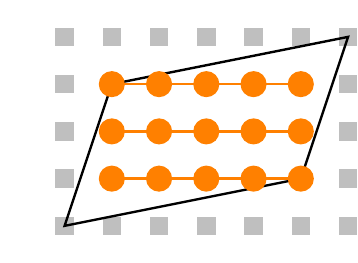
\begin{tikzpicture}[scale=0.6]\vspace{0.5cm}
\hspace{1em}
\foreach \x in {0,...,6} {
    \foreach \y in {0,...,4} {
        \node at (\x,\y) [fill=lightgray, minimum width=2pt] {};   
    }
}
\draw[line width=0.3mm, black] (0,0) -- (1,3) -- (6,4) -- (5,1) -- cycle;

\draw[line width=0.3mm, orange] (1,1) -- (5,1);
\draw[line width=0.3mm, orange] (1,2) -- (5,2);
\draw[line width=0.3mm, orange] (1,3) -- (5,3);


\foreach \x in {1,...,5} {
    \node at (\x,1) [circle, fill=orange, minimum width=3pt] {};
    \node at (\x,2) [circle, fill=orange, minimum width=3pt] {};
    \node at (\x,3) [circle, fill=orange, minimum width=3pt] {};
}
\end{tikzpicture}
\end{minipage}%
% --------- 2P ---------
\begin{minipage}[b]{0.33\textwidth}
\centering
\begin{tikzpicture}[scale=0.3]\vspace{0.5cm}
\foreach \x in {0,...,12} {
    \foreach \y in {0,...,8} {
        \node at (\x,\y) [circle, draw=white, fill=lightgray, minimum width=2.5pt] {};   
    }
}
\draw[line width=0.3mm, black] (0,0) -- (2,6) -- (12,8) -- (10,2) -- cycle;


\draw[line width=0.3mm, darklav] (1,2) -- (10,2);
\draw[line width=0.3mm, darklav] (1,3) -- (10,3);
\draw[line width=0.3mm, darklav] (2,5) -- (11,5);
\draw[line width=0.3mm, darklav] (2,6) -- (11,6);

\foreach \x in {1,...,10} {
    \node at (\x,2) [circle, fill=darklav, minimum width=3pt] {};
    \node at (\x,3) [circle, fill=darklav, minimum width=3pt] {};
}
\foreach \x in {2,...,11} {
    \node at (\x,5) [circle, fill=darklav, minimum width=3pt] {};
    \node at (\x,6) [circle, fill=darklav, minimum width=3pt] {};
}

\end{tikzpicture}
\end{minipage}%
% --------- 3P ---------
\begin{minipage}[b]{0.33\textwidth}
\raggedleft
\begin{tikzpicture}[scale=0.2]\vspace{0.5cm}
\foreach \x in {0,...,18} {
    \foreach \y in {0,...,12} {
        \node at (\x,\y) [circle, draw=white, fill=lightgray, minimum width=2.2pt] {};   
    }
}
\draw[line width=0.3mm, black] (0,0) -- (3,9) -- (18,12) -- (15,3) -- cycle;


\draw[line width=0.3mm, lightgreen] (1,3) -- (15,3);
\draw[line width=0.3mm, lightgreen] (2,6) -- (16,6);
\draw[line width=0.3mm, lightgreen] (3,9) -- (17,9);

\foreach \x in {1,...,15} {
    \node at (\x,3) [circle, fill=lightgreen, minimum width=3pt] {};
}
\foreach \x in {2,...,16} {
    \node at (\x,6) [circle, fill=lightgreen, minimum width=3pt] {};
}
\foreach \x in {3,...,17} {
    \node at (\x,9) [circle, fill=lightgreen, minimum width=3pt] {};
}
\end{tikzpicture}
\hspace{1em}
\end{minipage}
\caption{Lattice diameter segments in dilates of $P$ to visualize the values $n_i,\rem_i,r_i$ and $\blocks_i$.}
\label{fig:dilations-123}
\end{figure}
    %  \begin{figure}[ht!]
    %     \centering
    % \includegraphics[width=0.9\linewidth]{Figures/2.30_dilations.png}
    %     \caption*{}
    %     \label{fig:dilations-123}
    % \end{figure}
    
    For $i \in \{0, 1,2\}$ and $k \equiv i \pmod 3$ we partition the $\bu$-lattice lines that intersect $kR$ into $\blocks_i(k)$ $q$-blocks and $\rem_i$ remaining lattice lines. Here, $R$ and $2R$ have one $q$-block, and $3R$ has two $q$-blocks. These examples suffice to read off $n_i$, the number of lattice diameter lines per $q$-block, and $r_i$, the number of lattice diameter lines in the remaining $\rem_i$ lines, of $kR$ for any $k$. We get
  \begin{table}[h!]
    \centering
    \begin{tabular}{c|c|c|c|c}
    $i$ & $n_i$ & $\blocks_i(k)$ &$\rem_i$ & $r_i$\\ \hline \rule{0pt}{2.5ex}
    1 \hspace{1pt} & 3 & $\tfrac{1}{3}(2k+1)$ & 0 & 0 \\[3pt]
    2 & 2 & $\tfrac{1}{3}(2k-1)$ & 2 & 2 \\[3pt]
    0 & 1 & $\tfrac{1}{3}(2k)$ & 1 & \ 1.
    \end{tabular}\vspace{-1em}
    \caption*{}
\end{table}

\vspace{-1em}
Then, as in the proof of \Cref{thm:QP},
\begin{align*}
    \LD_P(k) = \LD_{R, (1,0)}(k) = n_i \cdot \blocks_i(k)+ r_i = \begin{cases}
         2k+1 & \text{if } k \equiv 1 \pmod 3,\\
            \frac{4}{3} k + \frac{4}{3} & \text{if } k \equiv 2 \pmod 3,\\
            \frac{2}{3} k + 1 & \text{if } k \equiv 0 \pmod 3.
    \end{cases}
\end{align*}
    
\end{example}

 We conjecture that counting lattice diameter segments or more generally counting $\ell$-slices of $P$ that contain the most lattice points among all $\ell$-dimensional slices of $P$ have a similar behavior under dilation of $P$. More precisely:
 
\begin{conjecture}
   Let $P$ be a lattice $d$-polytope, and $\ell \in [d]$. Define $\LD_P^{\ell}(k)$ as the number of $\ell$-dimensional slices of $P$ that contain the most lattice points among all $\ell$-dimensional slices of $P$. Then there exists a positive integer $q$ such that $\LD_P^{\ell}:\N_{\geq q} \to \N$ agrees with a quasi-polynomial function of degree $d-\ell$.
\end{conjecture}

A proof would require new ideas. For example, in many parts of our proof we rely on the fact that for every diameter direction, lattice diameter segments exist that pass through vertices. As shown in \Cref{ex:LD-3d-interior} this does not hold when $d \geq 3$. Furthermore, the relation between the number of lattice points on an $\ell$-slice and its normalized volume, as described in \Cref{lem:nvol}, is more subtle in higher dimensions.